\documentclass[a4paper,11pt]{book}
\usepackage{fullpage}
\usepackage{amsmath}
\usepackage{amssymb}
\usepackage{amstext}
\usepackage{array}

\usepackage{tikz-qtree,tikz-qtree-compat}
\usepackage{tikz}
\usetikzlibrary{shapes.geometric}
\usetikzlibrary{shapes.multipart}
\usetikzlibrary{shadows}
\usetikzlibrary{positioning}
\usetikzlibrary{trees}
\usetikzlibrary{arrows}


\newlength{\OUmatrixSepWidth}
\newcommand{\OUsetMatrixSepWidth}[1]{%
	\settowidth{\OUmatrixSepWidth}{#1}%
}


\title{Algorithm Design and Analysis (ECS 122A)\\Study Guide}
\author{Davis Computer Science Club\\
	Tutoring Committee
}
\date{Spring Quarter 2015}



\begin{document}

\makeatletter
\begin{titlepage}
	
\noindent \rule{\textwidth}{1pt}

\vspace{1cm}

\noindent {\LARGE \bfseries \@title}

\vspace{1cm}

\noindent \rule{\textwidth}{1pt}

\vspace{1cm}

\noindent	{\Large \@author }

\par\vspace*{\fill}
\begin{flushright}
	Spring Quarter 2015
\end{flushright}
\end{titlepage}

\tableofcontents
\newpage

% 
% ASYMPTOTIC NOTATION
%
\section{Asymptotic Notation}
% Big O
\subsection{O-Notation (Big O)}
\textbf{Notation:} 
$$f(n) \in O(g(n))$$
\textbf{Formal Definition:}\\
For a given function $g(n)$, $O(g(n))$ is the set of functions for which there exists positive constants $c$ and $n_0$ such that $0 \leq f(n) \leq c \cdot g(n)$ for all $n \geq n_0$.
$$
O(g(n)) = \{ f(n) : \exists \text{ } c, n_0 \text{ s.t. } 0 \leq f(n) \leq c \cdot g(n) \text{ } \forall \text{ } n \geq n_0 \}
$$
\textbf{Informal Definition:}\\
The function $g(n)$ is an asymptotic upper bound for the function $f(n)$ if there exists constants $c$ and $n_0$ such that $0 \leq f(n) \leq c \cdot g(n)$ for $n \geq n_0$.\\\\
Another way to perceive Big O notation is that for $f(n) \in O(g(n))$, the function $f$'s asymptotic\footnote{Asymptotic: As given variable approaches infinity.} growth is no faster than that of function $g$'s.\\\\
\textbf{Limit Definition:}
$$ 
\lim\limits_{n \to \infty} \frac{f(n)}{g(n)} < \infty
$$
\newpage
\subsubsection{Example}
\textbf{Prove that asymptotic upper bound of $f(n) = 2n+10$ is $g(n) = n^2$}.
\begin{eqnarray*}
	0 \leq f(n) &\leq& c \cdot g(n) \text{ for } n \geq n_0\\
	0 \leq 2n + 10 &\leq& c \cdot n^2 \text{ for } n \geq n_0
\end{eqnarray*}
Arbitrarily choose $c$ and $n_0$ values. Simplest is to turn one of the variables into the value $1$ and solve. For this example, we will assign the value 1 to $n_0$.
\begin{eqnarray*}
	0 \leq 2n + 10 &\leq& c \cdot n^2 \text{ for } n \geq 1\\
	2(1) + 10 &\leq& c \cdot (1)^2\\
	12 &\leq& c
\end{eqnarray*}
By picking $n_0 = 1$ and $c = 12$, the inequality of $2n+10 \leq 12n^2$ will hold true for all $n \geq 1$. Since there exists a constant $c$ and $n_0$ that fulfill this inequality, we have proven that $f(n) = 2n+10 = O(n^2)$.
\newpage

% Little O
\subsection{o-Notation (Little O)}
\textbf{Notation:}
$$
f(n) \in o(g(n))
$$
\textbf{Formal Definition:}\\
For a given function $g(n)$, $o(g(n))$ is the set  of functions for which every positive constant $c > 0$, there exists a constant $n_0 > 0$ such that $0 \leq f(n) \leq c \cdot g(n)$ for all $n \geq n_0$.
$$
o(g(n)) = \{ f(n) : \exists \text{ } n_0 \text{ s.t. } 0 \leq f(n) \leq c \cdot g(n) \text{ } \forall \text{ } n \geq n_0, c \geq 0 \}
$$
\textbf{Informal Definition:}\\
The function g(n) is an upper bound that is not asymptotically tight. For all positive constant values of $c$, there must exists a constant $n_0$ such that $0 \leq f(n) \leq c \cdot g(n)$ for all $n \geq n_0$. The value of $n_0$ may not depend on n, but may depend on $c$.\\\\
Another way to perceive Little O notation is that for $f(n) \in o(g(n))$, the function $f$'s asymptotic growth is strictly less than that of the function $g$'s. In this sense, Little O can be seen as a ``stronger" bound in comparison to Big O. By proving that a function is an element of Little O, it also proves that the function is an element of Big O.\\\\
\textbf{Limit Definition:}
$$
\lim\limits_{n\to\infty} \frac{f(n)}{g(n)} = 0
$$
\newpage
\subsubsection{Example}
\textbf{Prove that $f(n) = 2n$ has an upper bound $o(n^2)$.}
\begin{eqnarray*}
	0 \leq c \cdot g(n) &\leq& f(n) \text{ for } n \geq n_0\\
	0 \leq c \cdot 2n &\leq& n^2 \text{ for } n \geq n_0\\
	2c &\leq& n \text{ for } n \geq n_0\\
	2c &\leq& n_0
\end{eqnarray*}
For Little O to hold true, the inequality needs to hold true for all $c > 0$ and for all $n > n_0$. From simplifying the inequality, we assert that the inequality will hold true as long as the value of $n_0$ is twice the value of $c$. Given that they are both constants, then there exists a constant value of $n_0$ for all positive constant $c$ that fulfill this inequality.\\\\
Another method to solve this problem is to use the limit definition.
\begin{eqnarray*}
	&\lim\limits_{n\to\infty}& \frac{2n}{n^2}\\
	&\lim\limits_{n\to\infty}& \frac{2}{n} = 0	
\end{eqnarray*}

\subsubsection{Example}
\textbf{Prove that $f(n) = 2n^2$ does not have the upper bound $o(n^2)$.}
\begin{eqnarray*}
	0 \leq c \cdot g(n) &\leq& f(n) \text{ for } n \geq n_0\\
	0 \leq c \cdot 2n^2 &\leq& n^2 \text{ for } n \geq n_0\\
	2c &\leq& 1\text{ for } n \geq n_0
\end{eqnarray*}
For a function to have the Little O bound, the inequality must hold true for all positive $c$. However, simplification of the inequality asserts that the inequality will only hold true for all $c < \frac{1}{2}$. Therefore, $f(n) = 2n^2$ does not have the upper bound $o(n^2)$.
\newpage

% Big Omega
\subsection{$\Omega$-Notation (Big Omega)}
\textbf{Notation:}
$$
f(n) \in \Omega(g(n))
$$
\textbf{Formal Definition:}\\
For a given function $g(n)$, $\Omega(g(n))$ is the set of functions for which there exists positive constants $c$ and $n_0$ such that $0 \leq c \cdot g(n) \leq f(n)$ for all $n \geq n_0$.
$$
\Omega(g(n)) = \{ f(n) : \exists \text{ } c, n_0 \text{ s.t. } 0 \leq c \cdot g(n) \leq f(n) \text{ } \forall \text{ } n \geq n_0 \}
$$
\textbf{Informal Definition:}\\
The function $g(n)$ is an asymptotic lower bound for the function $f(n)$ if there exists constants $c$ and $n_0$ such that $0 \leq c \cdot g(n) \leq f(n)$ for $n \geq n_0$.\\\\
\textbf{Limit Definition:}
$$
\lim\limits_{n \to \infty} \frac{f(n)}{g(n)} > 0
$$
\newpage
\subsubsection{Example}
\textbf{Prove that the asymptotic lower bound of $f(n) = 8n^2$ is $g(n) = n$.}
\begin{eqnarray*}
	0 \leq c \cdot g(n) &\leq& f(n) \text{ for } n \geq n_0\\
	0 \leq c \cdot n &\leq& 8n^2 \text{ for } n \geq n_0
\end{eqnarray*}
Arbitrarily choose $c$ and $n_0$ values. Simplest is to turn one of the variables into the value $1$ and solve. For this example, we will assign the value 1 to $c$.
\begin{eqnarray*}
	0 \leq n &\leq& 8n^2 \text{ for } n \geq n_0\\
		   (n_0) &\leq& 8(n_0)^2\\
		   1 &\leq& 8n_0\\
		   \frac{1}{8} &\leq& n_0
\end{eqnarray*}
By picking $n_0 = 1$ and $c = 1$, the inequality of $n \leq 8n^2$ will hold true for all $n \geq 1$. Since there exists a constant $c$ and $n_0$ that fulfill this inequality, we have proven that $f(n) = n^2 = \Omega(n)$.
\newpage

% Little Omega
\subsection{$\omega$-Notation (Little Omega)}
\textbf{Notation:}
$$
f(n) \in \omega(g(n))
$$
\textbf{Formal Definition:}\\
For a given function $g(n)$, $\omega(g(n))$ is the set  of functions for which every positive constant $c > 0$, there exists a constant $n_0 > 0$ such that $0 \leq c \cdot g(n) \leq f(n)$ for all $n \geq n_0$.
$$
\omega(g(n)) = \{ f(n) : \exists \text{ } n_0 \text{ s.t. } 0 \leq c \cdot g(n) \leq f(n) \text{ } \forall \text{ } n \geq n_0, c \geq 0 \}
$$
\textbf{Informal Definition:}\\
The function g(n) is a lower bound that is not asymptotically tight. For all positive constant values of $c$, there must exists a constant $n_0$ such that $0 \leq c \cdot g(n) \leq f(n)$ for all $n \geq n_0$. The value of $n_0$ may not depend on n, but may depend on $c$.\\\\
Another way to perceive Little $\omega$ notation is that for $f(n) \in \omega(g(n))$, the function $f$'s asymptotic growth is strictly greater than that of the function $g$'s. In this sense, Little $\omega$ can be seen as a ``stronger" bound in comparison to Big $\Omega$. By proving that a function is an element of Little $\omega$, it also proves that the function is an element of Big $\Omega$.\\\\
\textbf{Limit Definition:}
$$
\lim\limits_{n\to\infty} \frac{f(n)}{g(n)} = \infty
$$
\newpage

% Theta
\subsection{$\Theta$-notation}
\textbf{Notation:}\\
$$
f(n) \in \Theta(g(n))
$$
\textbf{Formal Definition:}\\
For a given function $g(n)$, $\Theta(g(n))$ is the set of functions for which there exists positive constants $c_1$, $c_2$, and $n_0$ such that $0 \leq c_1 \cdot g(n) \leq f(n) \leq c_2 \cdot g(n)$ for all $n \geq n_0$.
$$
\Theta(g(n)) = \{ f(n) : \exists \text{ } c_1, c_2, n_0 \text{ s.t. } 0 \leq c_1 \cdot g(n) \leq f(n) \leq c_2 \cdot g(n) \text{ } \forall \text{ } n \geq n_0 \}
$$
\textbf{Informal Definition:}\\
The function g(n) is an asymptotic tight bound for the function f(n) if there exists constants $c_1$, $c_2$, and $n_0$ such that $0 \leq c_1 \cdot g(n) \leq f(n) \leq c_2 \cdot g(n)$ for $n \geq n_0$.\\\\
\textbf{Limit Definition:}\\
$$
\lim\limits_{n\to\infty} \frac{f(n)}{g(n)} \in \mathbb{R}_{>0}
$$
\newpage

%
% RECURRENCE RELATIONS
%
\chapter{Recurrence Relations}

\section{Recurrence Relations}
A recurrence relation is an equation that recursively defines a sequence of values. After the initial terms are given, each subsequent term is defined as a function of the previous terms.

\subsection{Fibonacci}
Fibonacci is an example of a recurrence relation.
$$
F_n = \begin{cases}
	F_{n-1} + F_{n-2}, &  n \geq 2\\
	1, & n = 1\\
	0, & n = 0
\end{cases}
$$
The first two terms are defined while the subsequent terms are a function of the two previous.

\subsection{Solving Recurrence Relations}
\begin{itemize}
	\item Substitution Method
	\item Recursion-Tree Method
	\item Master Method
\end{itemize}

\subsection{Substitution Method}
\begin{enumerate}
	\item Guess the bounds.
	\item Apply mathematical induction to prove the bounds. 
\end{enumerate}

\subsubsection{Example}
\textbf{Find the asymptotic upper bound for the following function:}
$$
T(n) \begin{cases}
	2T(n-1) + 1, & n \geq 1\\
	1, & n = 0
	\end{cases}
$$
\textbf{Guess}
$$T(n) \in O(2^n)$$
\textbf{Inductive Basis}
\begin{eqnarray*}
	T(0) &=& 2^0\\
	&=& 1
\end{eqnarray*}
\textbf{Inductive Hypothesis}\\
Assume that $T(n) = 2^n$ holds true for all $n = k$.\\\\
\textbf{Inductive Step}
\begin{align*}
T(n)	&=	2T(n-1) + 1						&& \text{Base equation}\\
		&= 	2T((k+1) - 1) + 1				&& \text{Substitute n with } k+1\\
		&=	2T(k) + 1						&& \text{Simplify parameters to T(n)}\\
		&=  2(2^k) + 1						&& \text{Substitute T(n) with inductive hypothesis}\\
		&=  2^{k+1} + 1						&& \text{Property of exponents}\\
&											&& \text{Q.E.D}
\end{align*}

%
%
%
\chapter{Divide and Conquer Paradigm}
\newpage

\section{Steps}

\begin{enumerate}
	\item \textbf{Divide} the problem into a number of independent subproblems.
	\item \textbf{Conquer} the subproblems by solving them recursively. 
	\item \textbf{Combine} the solutions of the subproblems into the solution of the original problem. 
\end{enumerate}
\newpage


\section{Case Study: Fibonacci Sequence}

\subsection*{Theorem}

\subsubsection*{Fibonacci Sequence Starting with 0}
Sequence: 0, 1, 1, 2, 3, 5, 8, 13, 21, 34, ...
\[
\begin{bmatrix}
F_{n}\\
F_{n-1}
\end{bmatrix}
=
\begin{bmatrix}
1 & 1\\
1 & 0
\end{bmatrix}^{n-1}
\begin{bmatrix}
F_{0}\\
F_{1}
\end{bmatrix}
\]

\subsubsection*{Fibonacci Sequence Starting with 1}
Sequence: 1, 1, 2, 3, 5, 8, 13, 21, 34, ...
\[
\begin{bmatrix}
F_{n}\\
F_{n-1}
\end{bmatrix}
=
\begin{bmatrix}
1 & 1\\
1 & 0
\end{bmatrix}^{n-1}
\begin{bmatrix}
F_{1}\\
F_{2}
\end{bmatrix}
\]

\subsection*{Derivation}
\begin{eqnarray*}
\begin{bmatrix}
	F_n\\
	F_{n-1}
\end{bmatrix}	
&=&
\begin{bmatrix}
	1 & 1\\
	1 & 0
\end{bmatrix}
\begin{bmatrix}
	F_{n-1}\\
	F_{n-2}
\end{bmatrix}\\
&=&
\begin{bmatrix}
	1 & 1\\
	1 & 0
\end{bmatrix}
\begin{bmatrix}
	1 & 1\\
	1 & 0
\end{bmatrix}
\begin{bmatrix}
	F_{n-2}\\
	F_{n-3}
\end{bmatrix}\\
&=&
\begin{bmatrix}
	1 & 1\\
	1 & 0
\end{bmatrix}
\begin{bmatrix}
	1 & 1\\
	1 & 0
\end{bmatrix}
\begin{bmatrix}
	1 & 1\\
	1 & 0
\end{bmatrix}
\begin{bmatrix}
	F_{n-3}\\
	F_{n-4}
\end{bmatrix}\\
&=&
\begin{bmatrix}
	1 & 1\\
	1 & 0
\end{bmatrix}^4
\begin{bmatrix}
	F_{n-4}\\
	F_{n-5}
\end{bmatrix}\\
&=&
\begin{bmatrix}
	1 & 1\\
	1 & 0
\end{bmatrix}^{n-1}
\begin{bmatrix}
	F_{0}\\
	F_{1}
\end{bmatrix}\\
\end{eqnarray*}
$$\text{To verify, let's choose } n = 5$$
\begin{eqnarray*}
	\begin{bmatrix}
		F_{5}\\
		F_{4}
	\end{bmatrix}
	&=&
	\begin{bmatrix}
		1 & 1\\
		1 & 0
	\end{bmatrix}^4
	\begin{bmatrix}
		F_{0}\\
		F_{1}
	\end{bmatrix}\\
		&=&
		\begin{bmatrix}
			5 & 3\\
			3 & 2
		\end{bmatrix}
		\begin{bmatrix}
			0\\
			1
		\end{bmatrix}\\
	&=&
	\begin{bmatrix}
		3\\
		2
	\end{bmatrix}
\end{eqnarray*}
$$
\text{The fifth Fibonacci number (assuming that the sequence starts at 0) is 3.}
$$

\subsection*{Recurrence Relation}
$$T(n) = T(\frac{n}{2}) + O(1)$$

\subsection*{Complexity}
$$T(N) \in \Theta(lg(n))$$
\newpage

\section{Case Study: Merge Sort}

\subsection*{Steps}

\begin{enumerate}
	\item \textbf{Divide} the list of n elements into two sublists with $\frac{n}{2}$ elements each.
	\item \textbf{Conquer} the sublists by sorting the two sublists recursively using merge sort. When the sublists are of size 1, it becomes sorted.
	\item \textbf{Combine} the elements of the two sublists by mering them in a sorted sequence.
\end{enumerate}

\subsection*{Recurrence Relation}
$$
T(n) = \begin{cases}
2T\left(\frac{n}{2}\right) + cn, & n \geq 2\\
c, & n = 1
\end{cases}
$$

\subsection*{Complexity}
$$
T(n) = \Theta(n \cdot lg(n))
$$

%\subsection{Example}
%\textbf{Show the steps of sorting the following list using merge sort: $\{ 13, 82, 72, 100, 25, 48, 71, 14 \}$}
\newpage

\section{Case Study: Maximum Subarray}

\subsection*{Steps}

\begin{enumerate}
	\item Divide the array in half into two subarrays (left subarray and right subarray).
	\item Recursively repeat this process until each subarray consists of only one element. At this point, the maximum sum of each subarray is the single element.
	\item Calculate the maximum sum for the cross section.
	\begin{enumerate}
		\item Start from the mid-point of the subarray.
		\item Sum up all numbers from the mid-point to the first element. Whenever the sum exceeds its previous value, that value becomes the left sum.
		\item Sum up all numbers from the mid-point+1 to the last element. Whenever the sum exceeds its previous value, that values becomes the right sum.
		\item The summation of the left sum and the right sum becomes the maximum sum for the cross section. Note: If all the elements in the subarrays are negative, then the left and right sum will return 0 by default.
	\end{enumerate}
	\item Compare the maximum sum from the left array, right array, and cross section. The largest of the three get returned.
\end{enumerate}

\subsection*{Recurrence Relation}
$$
T(n) = 2T(\frac{n}{2}) + \Theta(n)
$$

\subsection*{Complexity}
$$
T(n) \in \Theta(n \cdot lg(n))
$$

\newpage

\subsection{Example}
\textbf{Find the maximum subarray of the following array: $\{-2, 1, -3, 4, -1, 2, 1, -5, 4 \} $ }

\subsubsection*{Divide}
\begin{figure}[h]
	\centering
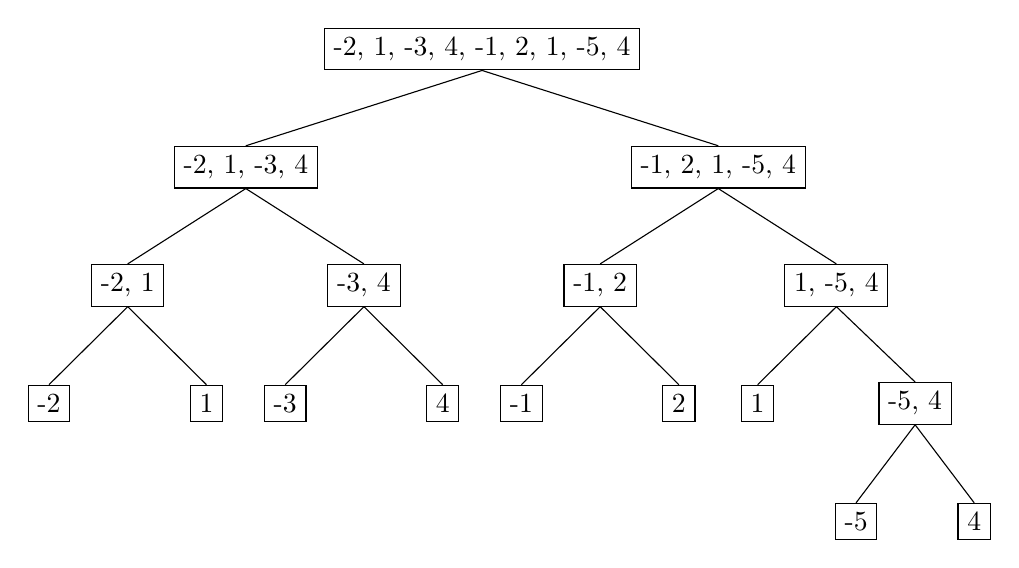
\begin{tikzpicture}[level/.style={sibling distance=60mm/#1}]
	\node [rectangle,draw] {-2, 1, -3, 4, -1, 2, 1, -5, 4}
		child {
			node [rectangle,draw] (a) {-2, 1, -3, 4}
				child {
					node [rectangle,draw] {-2, 1}
						child {
							node [rectangle, draw] {-2}
						}
						child {
							node [rectangle, draw] {1}
						}
				}
				child {
					node [rectangle,draw]{-3, 4}
					child {
						node [rectangle, draw] {-3}
					}
					child {
						node [rectangle, draw] {4}
					}
				}
		}
		child {
			node [rectangle,draw] (b) {-1, 2, 1, -5, 4}
				child {
					node [rectangle,draw]  {-1, 2}
						child {
							node [rectangle, draw] {-1}
						}
						child {
							node [rectangle, draw] {2}
						}
				}
				child {
					node [rectangle,draw]  {1, -5, 4}
						child {
							node [rectangle, draw]  {1}
						}
						child {
							node [rectangle, draw] {-5, 4}
								child {
									node [rectangle, draw] {-5}
								}
								child {
									node [rectangle, draw] {4}
								}
						}
				}
		};
\end{tikzpicture}
\end{figure}

\subsubsection*{Combine}
\begin{table}[h]
	\centering
	\begin{tabular}{| >{$}c<{$} | >{$}c<{$} |  >{$}c<{$} | >{$}c<{$} | >{$}c<{$} | >{$}c<{$} | >{$}c<{$} |}
		\hline
		\text{Depth}
			&	\text{Left Subarray}
			&	\text{Right Subarray}	
			&	\text{Max(Left)}	
			&	\text{Max(Right)}	
			&	\text{Max(Cross)}
			&	\text{Return}\\
		\hline
		4		
			&	\{ -5 \}	
			&	\{ 4 \}
			& 	-5
			&	4
			&	4
			&	4\\
		\hline
		3
			&	\{ -2 \}
			&	\{ 1 \}
			&	-2
			&	1
			&	1
			&	1\\
		\hline
			&	\{ -3 \}
			&	\{ 4 \}
			&	-3
			&	4
			&	4
			&	4\\
		\hline
			&	\{ -1 \}
			&	\{ 2 \}
			&	-1
			&	2
			&	2
			&	2\\
		\hline
			&	\{ 1 \}
			&	\{ -5, 4 \}
			& 	1
			&	4
			&	4
			&	4\\
		\hline
		2
			&	\{ -2, 1\}
			&	\{ -3, 4\}
			&	1
			&	4
			&	1
			&	4\\
		\hline
			&	\{ -1, 2 \}
			&	\{ 1, -5, 4 \}
			&	2
			&	4
			&	3
			&	4\\
		\hline
		1
			&	\{ -2, 1, -3, 4 \}
			&	\{ -1, 2, 1, -5, 4 \}
			&	4
			&	4
			&	6
			&	6\\
		\hline
	\end{tabular}
\end{table}
$$
\text{The maximum sum is 6 from indices 3 to 6.}
$$

\subsubsection*{Visualization of Finding the Max of Cross Section}
Taking depth = 1 with left subarray = $\{ -2, 1, -3, 4 \}$ and right subarray = $\{ -1, 2, 1, -5, 4 \}$.

\begin{minipage}[t]{0.5\linewidth}
	$$
	\text{Cross Section Left Sum}
	$$
	$$
	\{ -2, 1, -3, 4, \underbrace{-1}_{\text{Mid}}, 2, 1, -5, 4 \}
	$$
	$$
	\{ -2, 1, -3, 4, \underbrace{-1}_{\text{-1}}, 2, 1, -5, 4 \}
	$$
	$$
	\{ -2, 1, -3, \underbrace{4, -1}_{\text{3}}, 2, 1, -5, 4 \}
	$$
	$$
	\{ -2, 1, \underbrace{-3, 4, -1}_{\text{0}}, 2, 1, -5, 4 \}
	$$
	$$
	\{ -2, \underbrace{1, -3, 4, -1}_{\text{1}}, 2, 1, -5, 4 \}
	$$
	$$
	\{ \underbrace{-2, 1, -3, 4, -1}_{\text{-1}}, 2, 1, -5, 4 \}
	$$
	$$\text{Max Left Sum} = 3$$
\end{minipage}
\begin{minipage}[t]{0.5\linewidth}
	$$
		\text{Cross Section Right Sum}
	$$
	$$
	\{ -2, 1, -3, 4, -1, \underbrace{2}_{\text{Mid + 1}}, 1, -5, 5 \}
	$$
	$$
	\{ -2, 1, -3, 4, -1, \underbrace{2}_{\text{2}}, 1, -5, 5 \}
	$$
	$$
	\{ -2, 1, -3, 4, -1, \underbrace{2, 1}_{\text{3}}, -5, 5 \}
	$$
	$$
	\{ -2, 1, -3, 4, -1, \underbrace{2, 1, -5}_{\text{-2}}, 4 \}
	$$
	$$
	\{ -2, 1, -3, 4, -1, \underbrace{2, 1, -5, 4}_{\text{2}} \}
	$$
	$$
	\text{Max Right Sum} = 3
	$$
\end{minipage}




%
% APPENDIX
%
\chapter{Side Topics}
\newpage

\subsection{Solving Recurrence Relations with Induction}

\subsubsection{Example}
\textbf{Prove that the following systems of equations has the solution $T(n) = n \cdot lg(n)$.}
$$
T(n) \begin{cases}
	2T(\frac{n}{2}) + n, & n = 2^k \mbox{ for } k > 1\\
	2, & n = 2
\end{cases}
$$
\textbf{Basis}
\begin{eqnarray*}
T(2) &=& (2) \cdot lg(2)\\
	&=& 2 \cdot 1\\
	&=& 2
\end{eqnarray*}
\textbf{Inductive Hypothesis}\\
Assume that $T(n) = n \cdot lg(n)$ holds true for all $n = 2^k$.\\\\
\textbf{Inductive Step}
\begin{align*}
T(n)	&=	2T(\frac{n}{2}) + n						&& \text{Base equation}\\
		&= 	2T(\frac{2^{k+1}}{2}) + 2^{k+1}			&& \text{Substitute n with } 2^{k+1}\\
		&= 	2T(2^{k}) + 2^{k+1}						&& \text{Simplify parameters to function T(...)}\\
		&=	2(2^k \cdot lg(2^k)) + 2^{k+1}			&& \text{Inductive hypothesis}\\
		&=	2^{k+1} \left[ lg(2^k) + 1 \right]		&& \text{Distributive property}\\
		&=  2^{k+1} \left[ lg(2^k) + lg(2) \right]  && \text{Logarithmic identity}\\
		&= 	2^{k+1} \cdot lg(2^k \cdot 2)			&& \text{Logarithmic identity}\\
		&=  2^{k+1} \cdot lg(2^{k+1})				&& \text{Exponent property}\\
		&											&& \text{Q.E.D}
\end{align*}

\subsubsection{Example}
\textbf{Prove that the following systems of equations has the solution $T(n) = 2F(n) - 1$ where $F(n) = F(n-1) + F(n-2)$.}
$$
T(n) \begin{cases}
T(n-1) + T(n-2) + 1, & \mbox{if } n \geq 2\\
0, & \mbox{if } n = \{0,1\}
\end{cases}
$$
\textbf{Basis}
\begin{eqnarray*}
	T(0) &=& 1
\end{eqnarray*}
\textbf{Inductive Hypothesis}\\
Assume that $T(n) = F(n) - 1$ is true for all $n = k$.\\
\textbf{Inductive Step}
\begin{align*}
	T(n) 	&= T(n-1) + T(n-2) + 1					&& \text{Base equation}\\
	T(k+1) 	&= T((k+1) - 1) + T((k+1) - 2) + 1 		&& \text{Substitute n with k+1}\\
			&= T(k) + T(k-1) + 1					&& \text{Simplify parameters to function T(...)}\\
			&= (2F(k) - 1) + (2F(k-1) - 1) + 1		&& \text{Inductive hypothesis}\\
			&= 2F(k) + 2F(k-1) - 1					&& \text{Simplify equation}\\
			&= 2(F(k) + F(k-1)) - 1					&& \text{Distributive property}\\
			&= 2(F(k+1)) - 1						&& \text{Definition of function: } F(k+1) = F(k) + F(k-1)\\
			&= 2F(k+1) - 1							&& \text{Simplify}\\
			&										&& \text{Q.E.D}
\end{align*}


\end{document}